\section{Архитектура на системата}

\subsection{Конструкция на платформата}

\subsection{Платформа с четири ротора}
\FloatBarrier

Платформата \autoref{fig:drone_construction} е конструирана от два метални П-образни профила, сключващи прав ъгъл помежду си и имащи пресечна точка в средата.
В края на профилите се намира по един безчетков постояннотоков мотор (без обратна връзка).
Перките са свързани директно (без трансмисия) за въртящата ос на моторите.
Батерията и контролният модул са позиционирани в средата на платформата.
Батерията се намира под пресечната точка на профилите.
Управляващото устройство е над пресеччната точка на профилите
върху изработена, като част от проекта, платформа.

При този начин на организиране на хардуера центърът на тежеста лежи под пресечната точка на профилите.


\begin{figure}[htpb!]
    \centering
    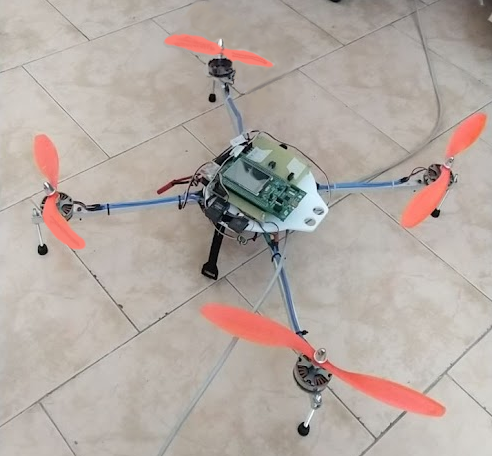
\includegraphics[width=0.5\textwidth]{drone_construction}
    \caption{Конструкция на платформата с четири ротора}
    \label{fig:drone_construction}
\end{figure}



\FloatBarrier
\subsection{Платформа за управление на ъгъл на завъртане}
\FloatBarrier

Платформата за управление на ъгъл на завъртане има за цел да ни позволи лесно и безаварийно да изпробваме алгоритмите за управление на ъгъл на завъртане.

Платфомрата \autoref{fig:balance_construction} е изградена от дърво.
Състои се от Т-образна основа с ограничители и въртяща част.
Основата е висока \(30cm\) и е съставена от два правоъгълни дървени профила (\(30x10x2.5cm\)), съединенин с винтове. 
Ограничителите ограничават максималния ъгъл, който въртящата част може да сключва с хоризонта в диапазона (\(\pm 40^{\circ}\)).
Оста на въртене представлява M8 болт.
Оста образува болтово съединение с основата, както и с лагерите на въртяащата част.
Въртящата част е съставена от правоъгълен дървен профил (\(60x2.5x3cm\)) с вложени два лагера 
(сачмен с дълбок канал \(8x22mm\), максимално статично натоварване \(138kg\) \cite{datasheet_bearing}),
като са пробити отвори за болтово съединяване на основите за безчетковите постояннотокови мотори,
както и отвори за болтово съединяване на основата на жироскопа и акселерометъра.
Останалите нужни компонении като \textit{ESC (Electronic Speed Controller)} за моторите са прикрепени към рамената на въртящата
част чрез кабелни превръзки (т.нар свински опашки), като е взето предвид балансиране на платформата
чрез разпределение на тежеста на допълнителните елементи.

\begin{figure}[htpb!]
    \centering
    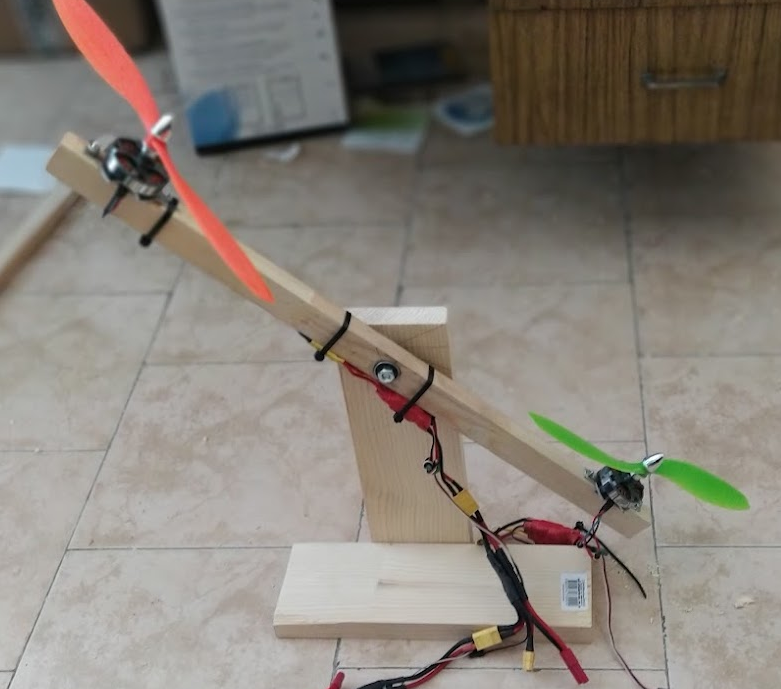
\includegraphics[width=0.7\textwidth]{balance_construction}
    \caption{Конструкция на платформата за управление на ъгъл}
    \label{fig:balance_construction}
\end{figure}

\FloatBarrier



\subsection{Софтуерна част}

\begin{figure}[htpb!]
    \centering
    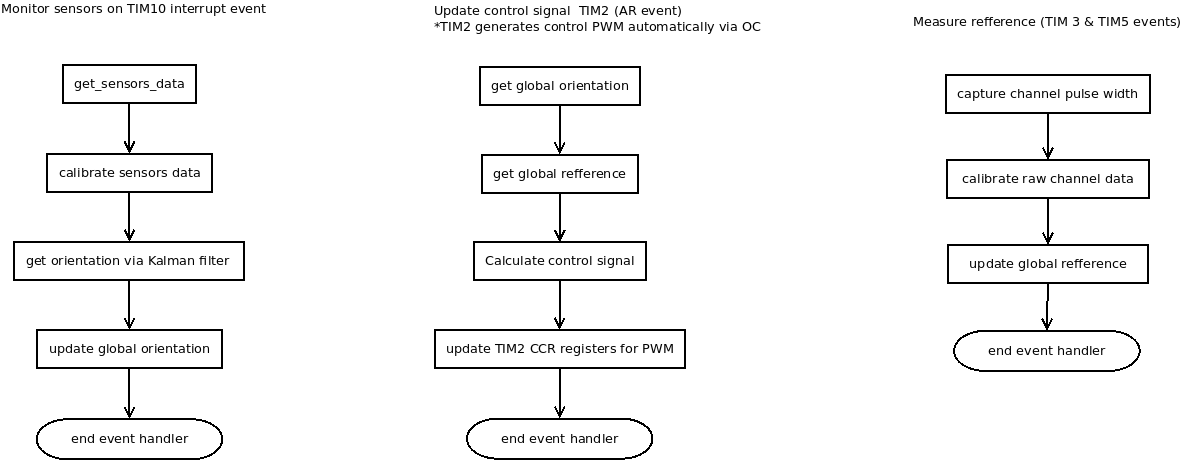
\includegraphics[width=1\textwidth]{main_events}
    \caption{Основни събития, касаещи управлението}
    \label{fig:main_events}
\end{figure}


\subsubsection{Модул stdperiph}

За управление на периферията са имплементирани отделни подмодули, всеки от които
е опростен API (Application Programming Interface) за управление на 
интегрираната периферия в микроконтролера. Всеки подмодул е отговорен само и
единсттвено за конкретното интегрирано периферно устройство, за което е създаден.
Интеграцията между периферните подмодули се осъществява отвън.

Подмодулите от този модул са отговорни за инициализиране и управление на
регистрите на интегрираната периферия. 

\subsubsection{Модул CMSIS}

CMSIS е стандарт на ARM за стандартни математически операции.
Той дефинира прототипите на функциите, както и множество
структури от данни за работа с матрици, вектори, тригонометрични и 
други математичски функции.

В проекта е интегрирана модифицирана CMSIS библиотека 
като част от модула за математика.

\subsubsection{Модул math}

Този модул предоставя функции за работа с числа, матрици и полиноми.
Като част от този модул е съставена опростена библиотека за конверсия,
която ще бъде използвана за интегриране с останалите модули.

\subsubsection{Модул control}

Този модул предоставя възможността за лесна инициализация,
конфигуриране и използване на средства за управление.
За момента в модула са имплементирани ПИД регулатор и ограничител.

\subsubsection{Модул специфични за проекта функции}

В този модул са изнесени подмодули и логически смислени наименования на изпълнявани процедури
за удобство и нагледност при писане на софтуера.
Подмодулите, имплементирани в този модул, са подмодул за филлтър на Калман,
подмодул за калибриране и компенсация на сензорни отмествания и други.